\documentclass[a4paper,english]{article}
\usepackage{graphicx}
%% Use utf-8 encoding for foreign characters
%%\usepackage[T1]{fontenc}
%%\usepackage[utf8]{inputenc}
%%\usepackage{babel}
%%
%%%% Vector based fonts instead of bitmaps
%%\usepackage{lmodern}
%%
%%%% Useful
%%%\usepackage{fullpage} % Smaller margins
%%\usepackage{enumerate}
%%
%%%% Theorem
%%\usepackage{amsthm}
%%
%%%% More math
%%\usepackage{amsmath}
%%\usepackage{amssymb}

%% Document Header
\title{Section2}
\author{Elliott Ashby}
\date{\today}

\begin{document}
    \maketitle
    \section{q1}
        If fabs is ommitted there may arise a situation where total is negative and therefore
        if $1.0e^{-13}$ is added to it would have the opposite effect on the inequality therefore
        not making the desired outcome. Essentially, if term and total are negative, the wrong 
        stopping condition is applied resulting in undesired results. (See Figure 1)
        \begin{figure}
            \caption{Incorrect stopping condition:}
            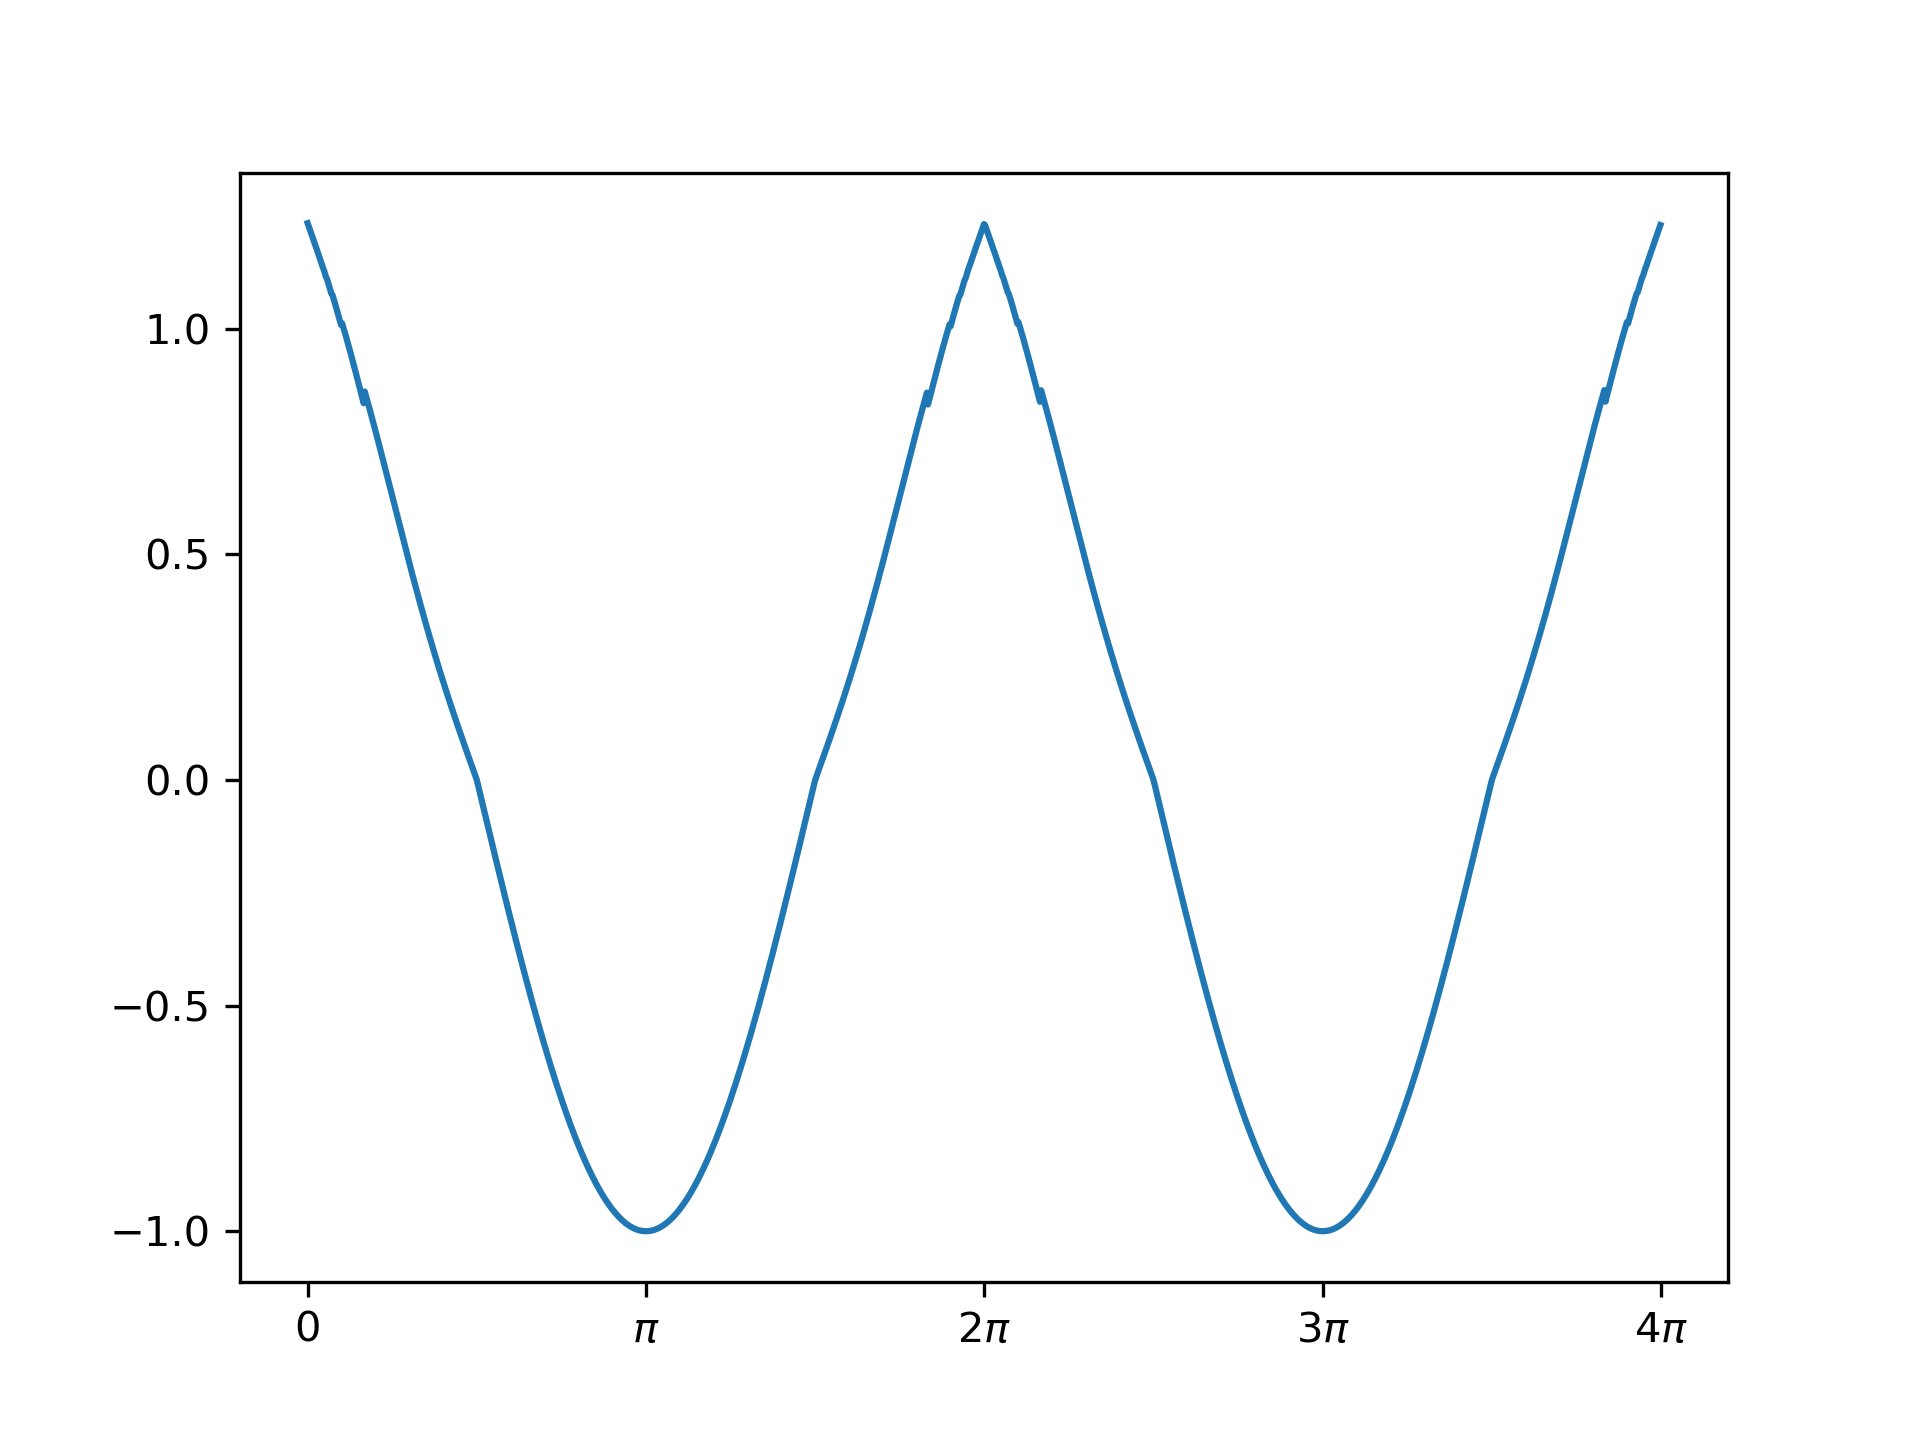
\includegraphics[scale=1]{./q1nofabs.png}
        \end{figure}
    \section{q2}
        
\end{document}
